\newpage
\section{Формат сообщений EAP-PSK}

Для простоты, EAP-PSK использует фиксированный формат собщений. Существует четыре различных типа EAP-PSK сообщений:

\begin{itemize}
\item Первый тип, который передается от сервера к Пиру;
\item Второй тип, который передается от Пира к серверу;
\item Третий тип, который передается от сервера к Пиру;
\item Четвертый тип, который отправляется от Пира к серверу. Так же это тип сообщений, которые Пир собирается отправить серверу в случае расширенной аутентификации. Так же это тип сообщений которые сервер будет отправлять Пиру в случае расширенной аутентификации: есть лишь небольшое отличие, в этом случаее EAP устанавливает в поле Code значение 1, в остальных случаях в это поле устанавливается значение 2.
\end{itemize}

Для ясности, весь EAP пакет, который инкапсулируется в сообщение EAP-PSK (то есть сообщение EAP-PSK плюс заголовок EAP), представлен на рисунках \ref{img:message_type1}, \ref{img:message_type2}, 14 и 18. %TODO

\subsection{EAP-PSK сообщение первого типа}

Первый тип сообщений отправляется сервером к Пиру. Формат данного сообщения представлен на рисунке \ref{img:message_type1}.

\begin{figure}[h!]
\center{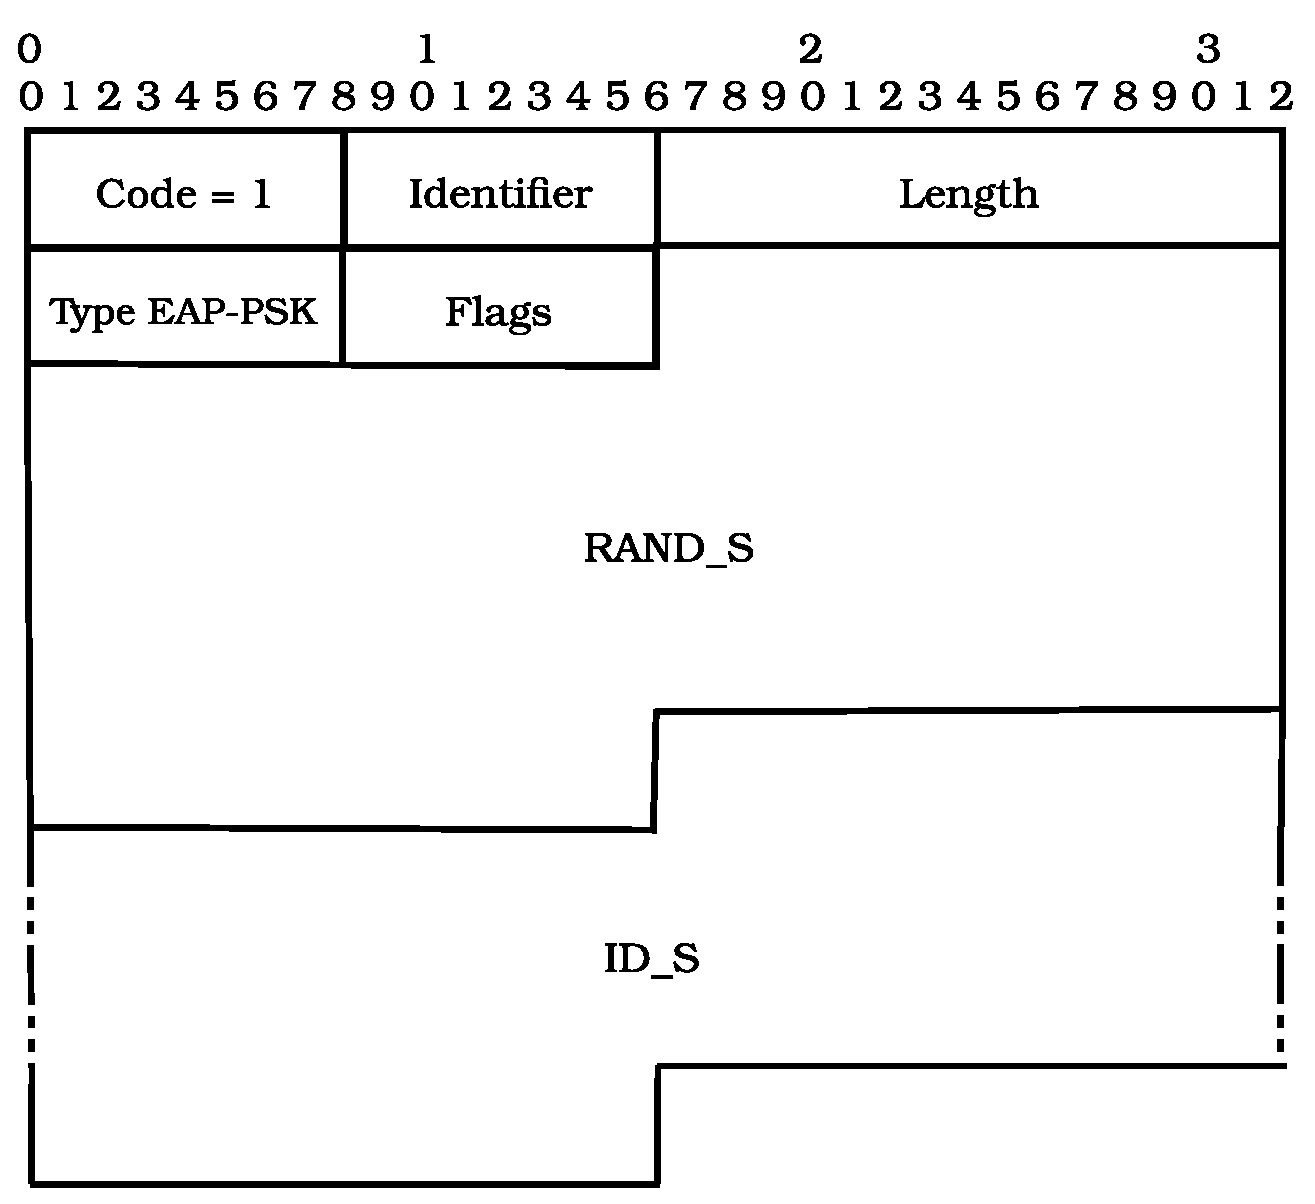
\includegraphics[width=0.9\linewidth]{./pictures/message_type1}}
\caption{Сообщение первого типа}
\label{img:message_type1}
\end{figure}

Так как IANA выделил методу EAP-PSK тип номер 47, в поле Type первого сообщения EAP-PSK, в отличии от остальныз, ДОЛЖНО помещаться значение 47.

Первое сообщение EAP-PSK состоит из:

\begin{itemize}
\item 1-байтового поля Flags;
\item 16-байтового случаного числа RAND\_S;
\item поле переменной длины, в котором передается NAI сервера: ID\_S. Длина данного поля вычисляется из поля Length пакета EAP. Длина NAI не должна превышать 966 байт. Это ограничение установлено для того, что бы избежать проблемы фрагментации данных (раздел 8.11).
\end{itemize}

Поле Flags имеет формат, представленный на рисунке \ref{img:flags_field}.

\begin{figure}[h!]
\center{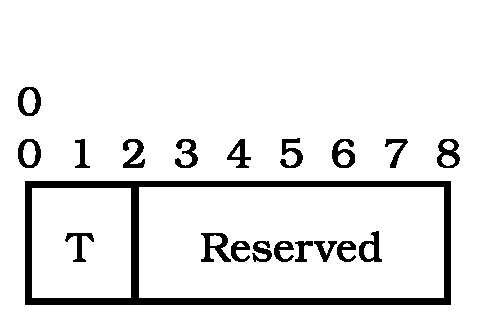
\includegraphics[width=0.9\linewidth]{./pictures/flags_field}}
\caption{Поле Flags EAP-PSK}
\label{img:flags_field}
\end{figure}

Поле Flags состоит из двух частей:

\begin{itemize}
\item первые два бита T показывают тип сообщения EAP-PSK:
\begin{itemize}
\item T = 0 для сообщений первого типа (раздел 5.1);
\item T = 1 для сообщений второго типа (раздел 5.2);
\item T = 2 для сообщений третьего типа (раздел 5.3);
\item T = 3 для сообщений четвертого типа (раздел 5.4) и последующих сообщений, которые могут отправляться в случае расширенной аутентификации.
\end{itemize}
\item остальные 6 бит зарезервированы. При передачи сообщения все они устанавливаются в 0, а при приеме игнорируются.
\end{itemize}

Одноразовый номер N (раздел 5.3) используется для того, что бы различать сообщения EAP-PSK, обмен которыми происходит при расширенной аутентификации, если все они имеет значение T = 3, то есть для четвертого и последующих сообщений.

\subsection{EAP-PSK сообщения второго типа}

EAP-PSK сообщения второго типа отправляется от Пира к серверу. Формат данного сообщения представлен на рисунке \ref{img:message_type2}.

\begin{figure}[h!]
\center{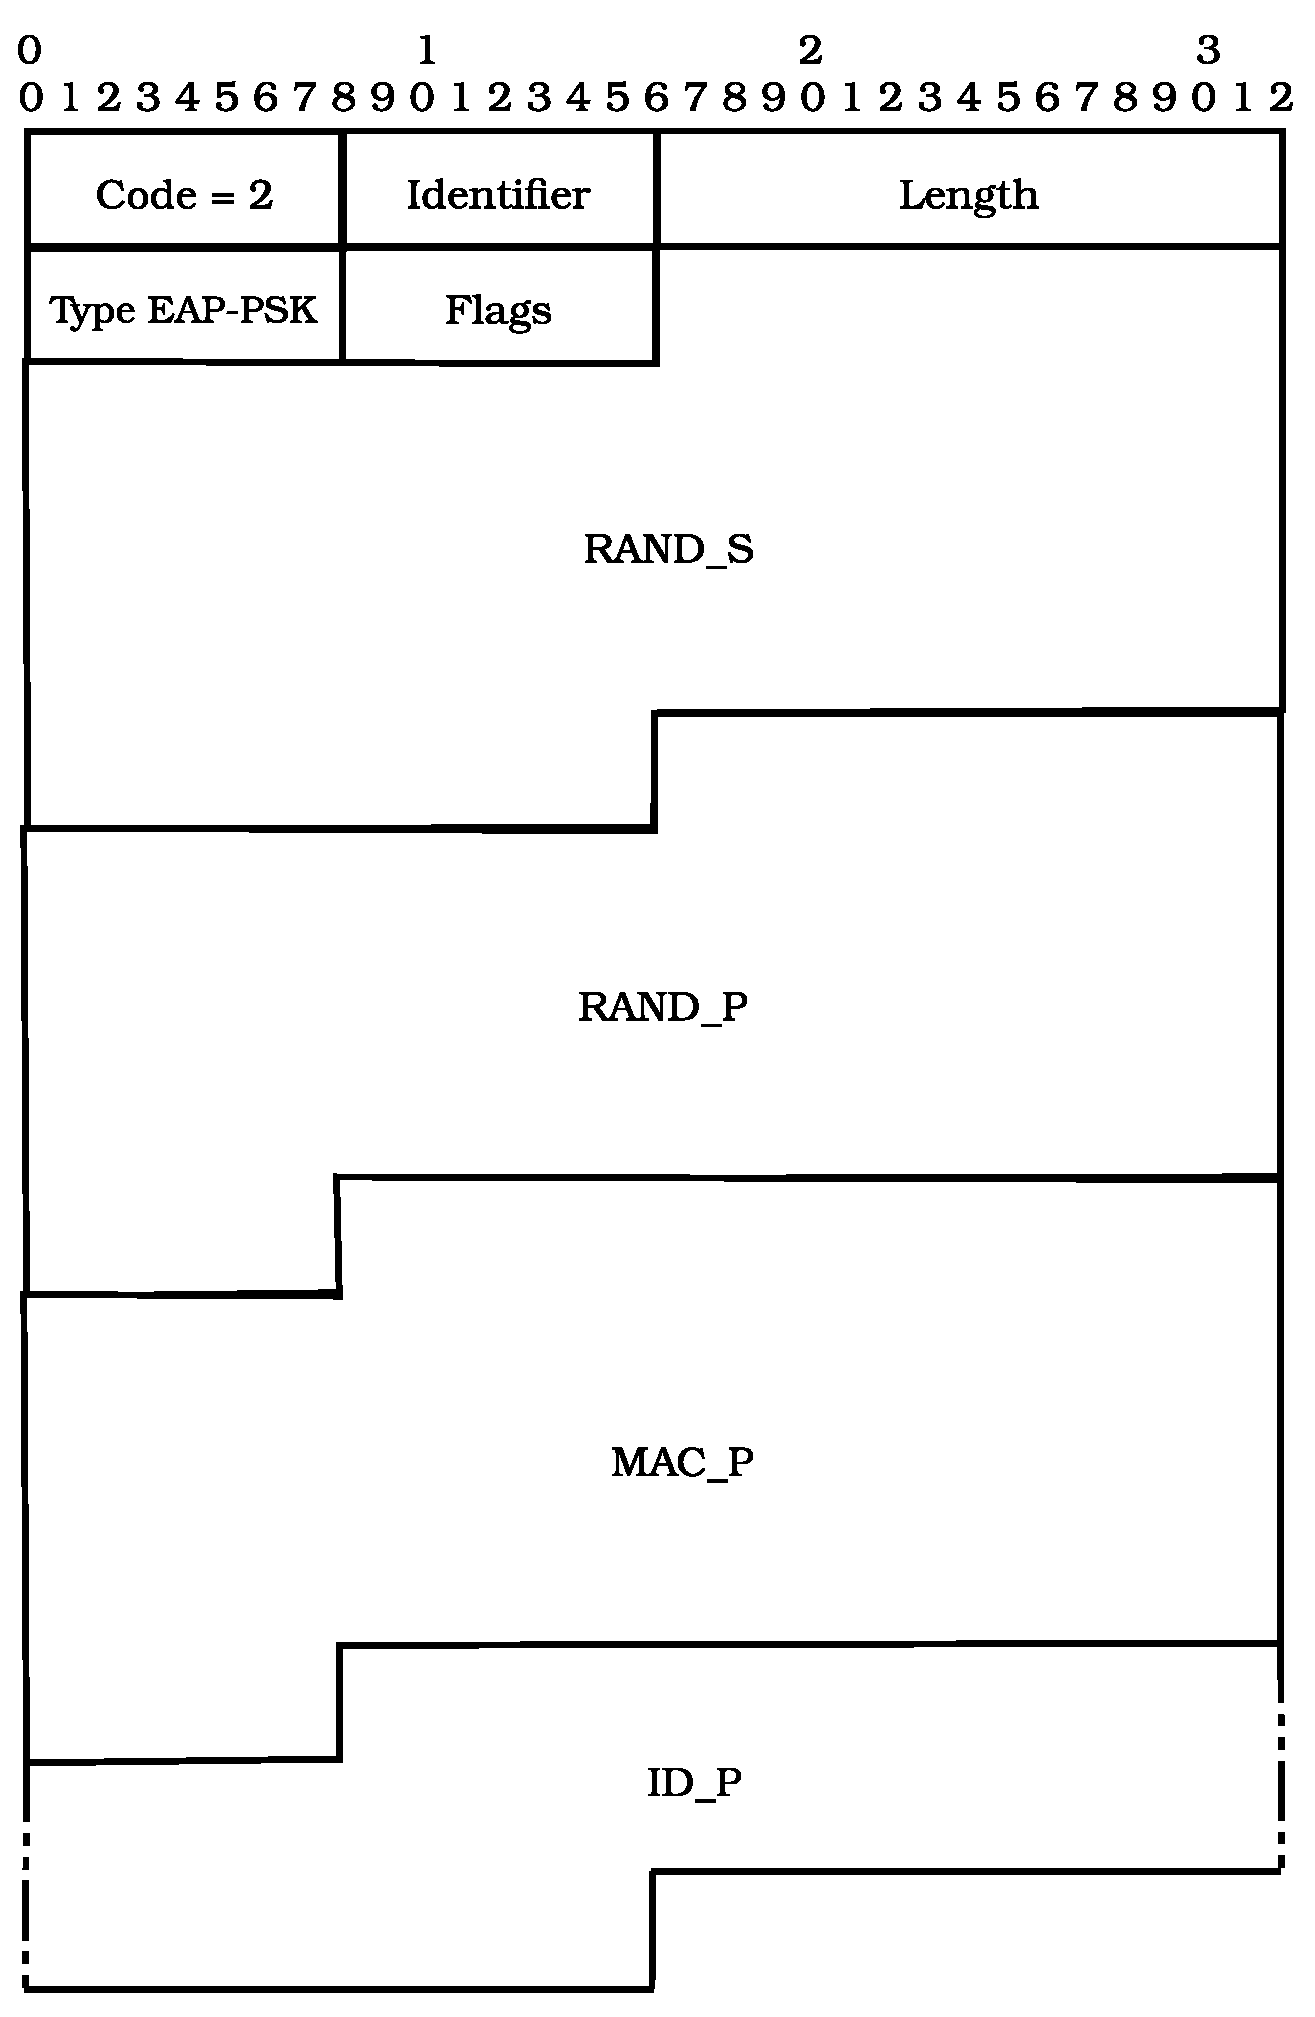
\includegraphics[width=0.9\linewidth]{./pictures/message_type2}}
\caption{Сообщение второго типа}
\label{img:message_type2}
\end{figure}

Второе сообщение EAP-PSK состоит из:

\begin{itemize}
\item 1-байтового поля Flags;
\item 16-байтового случаного числа, отправленное сервером в первом сообщении EAP-PSK (RAND\_S), которое служит идентификатором сессии;
\item 16-байтового случаного числа RAND\_P;
\item 16-байтового MAC: MAC\_P;
\item поле переменной длины, в котором передается NAI Пира: ID\_P. Длина данного поля вычисляется из поля Length пакета EAP. Длина NAI не должна превышать 966 байт. Это ограничение установлено для того, что бы избежать проблемы фрагментации данных (раздел 8.11).
\end{itemize}

Поле Flags имеет формат, представленный на рисунке \ref{img:flags_field}.

\subsection{EAP-PSK сообщения третьего типа}

Третий тип сообщений отправляется сервером к Пиру. Формат данного сообщения представлен на рисунке \ref{img:message_type3}.

\begin{figure}[h!]
\center{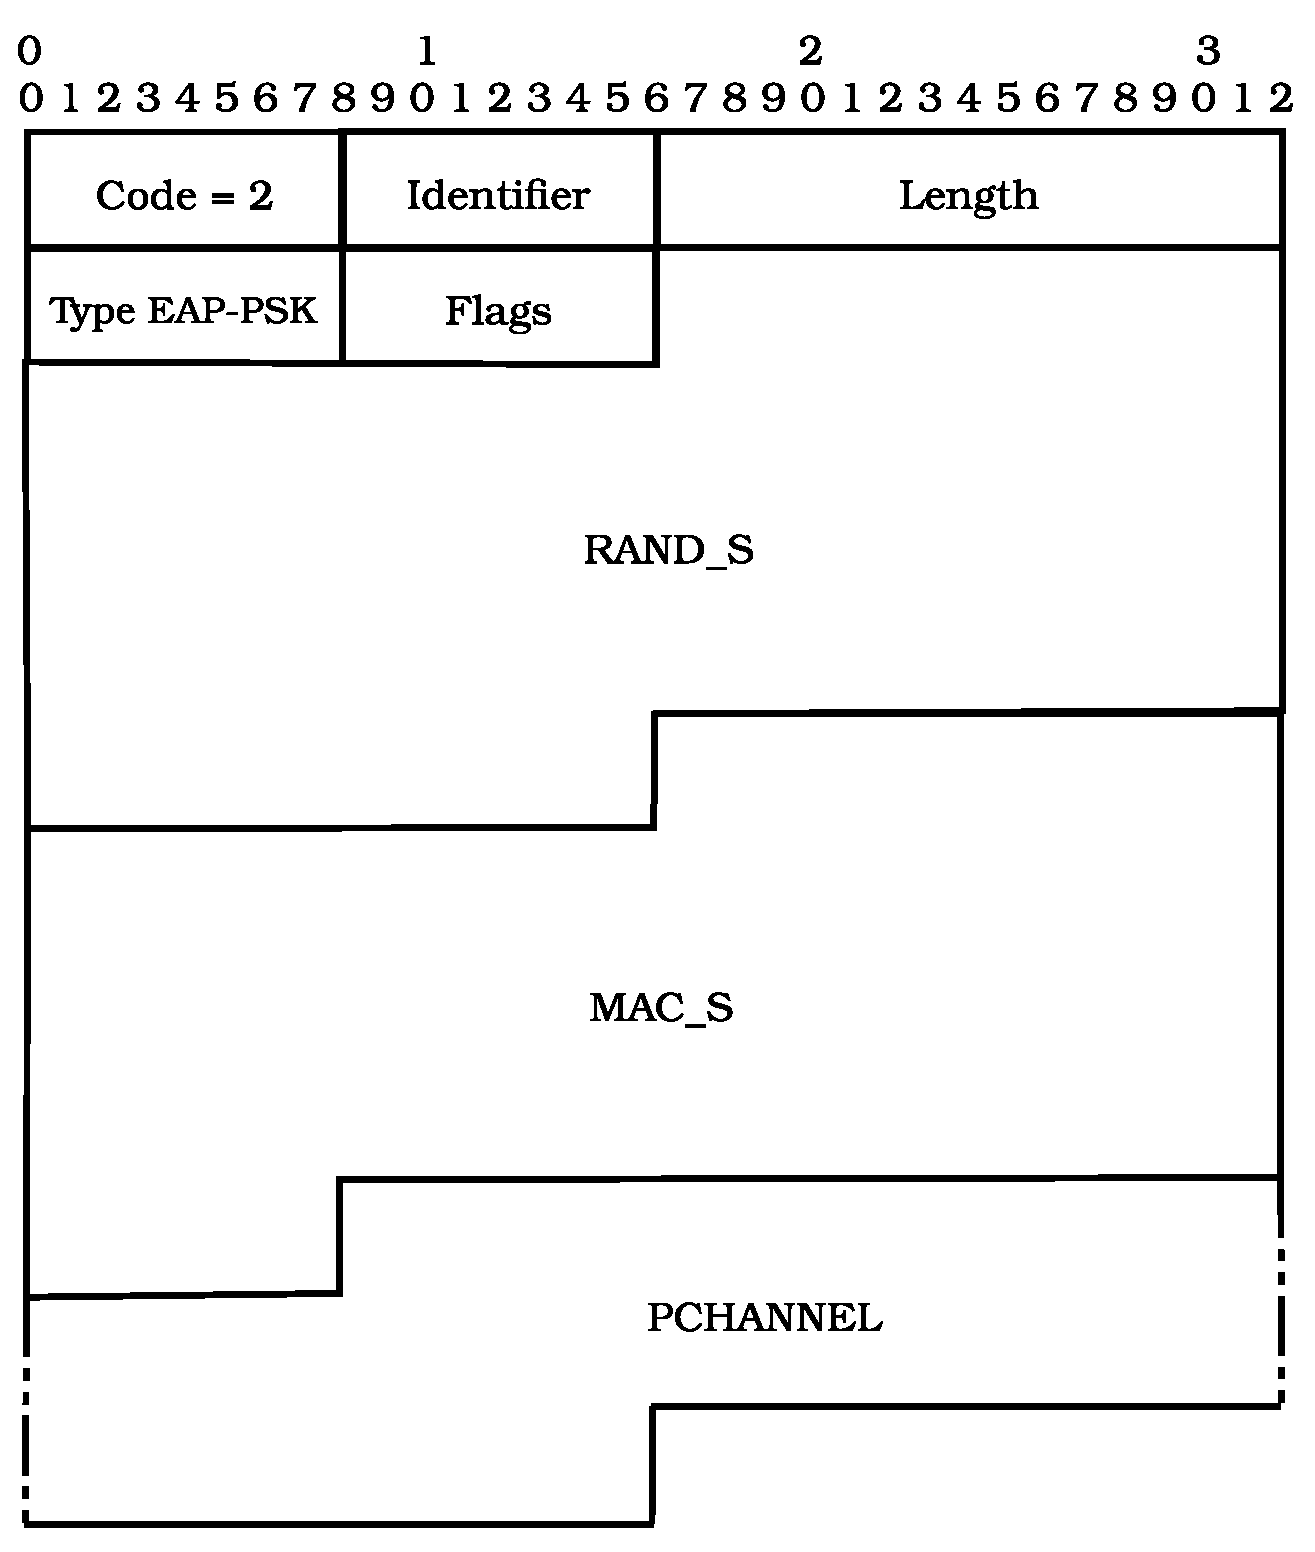
\includegraphics[width=0.9\linewidth]{./pictures/message_type3}}
\caption{Сообщение третьего типа}
\label{img:message_type3}
\end{figure}
